\chapter*{Background}

\section*{Air Quality Monitors}
\addcontentsline{toc}{section}{Air Quality Monitors}
Air quality monitors are used to collect sensor data from different sources in the air. \cite{GeneralAirQualityMonitor} Air quality monitors can specialize in one measuring unit in the air or have the functionality to measure several air quality factors, such as gas, particulate pollutants, CO2, VOCs, humidity or temperature. 

\subsection*{Privacy and Security in Air Quality Monitors}
\addcontentsline{toc}{section}{Privacy and Security in Air Quality Monitors}
General security 
Encryption etc

Considering the amount of information an air quality monitor can collect about an individual or a smart home, privacy leakage is a vulnerability. \cite{SecPrivSmartCity} 


\subsection*{Private Information Inference}
\addcontentsline{toc}{subsection}{Private Information Inference}


\subsection*{Passive network Eavesdropping}
\addcontentsline{toc}{subsection}{Passive network Eavesdropping}

\section*{Communication Protocols}
\addcontentsline{toc}{section}{Communication Protocols}
Air Quality Monitors exists with different functionality and therefore also communicate over different communication protocols. Wi-Fi is the most preferred protocol with Bluetooth and Zigbee following. \cite{saini2020indoor} As this thesis is delimited to air quality monitor devices that uses Wi-Fi, Bluetooth or Zigbee as communication protocols, the next subsections will elaborate on these protocols and specifications to be used further in this thesis through testing and analysis. 

\subsection*{IEEE 802.11 - Wi-Fi}
\addcontentsline{toc}{subsection}{IEEE 802.11 - Wi-Fi}
Wireless Fidelity (Wi-Fi) \cite{WiFiAlliance} is one of the worlds most used technology for communicating and is defined, developed and standarized by WiFi Alliance. \cite{WiFiAlliance} Wi-Fi is based on the standard IEEE 802.11 Wireless LAN set by IEEE Standard for Information Technology. \cite{WifiStandard} 

Wi-Fi packets transmitted follows the MAC frame format and is defined in Figure \ref{MACFrameFormat}. \cite{WifiStandard} 
\begin{figure}
    \centering
    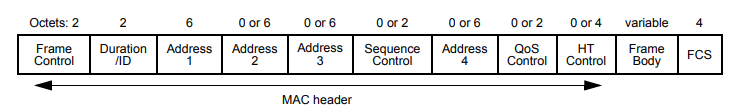
\includegraphics{figures/MACFrameFormat.png}
    \caption{MAC Frame Format \cite{WifiStandard}}
    \label{MACFrameFormat}
\end{figure}

\begin{itemize}
    \item Frame Control: 
    \item Duration/ID
    \item Address 1
    \item Address 2
    \item Address 3
    \item Sequence Control
    \item Address 4
    \item QoS Control
    \item HT Control
    \item Frame Body
    \item FCS
    
\end{itemize}

\subsection*{Bluetooth}
\addcontentsline{toc}{subsection}{Bluetooth}

\subsection*{Zigbee}
\addcontentsline{toc}{subsection}{Zigbee}